% #####################################################################
% #####################################################################
% ##                                                                 ##
% ##                             Lizenz:                             ##
% ##                         CC BY-NC-SA 3.0                         ##
% ##      http://creativecommons.org/licenses/by-nc-sa/3.0/de/       ##
% ##                                                                 ##
% #####################################################################
% ##   Diese Datei kann beliebig verändert werden, solange darauf    ##
% ##     hingewiesen wird, dass dieses Dokument ursprünglich von     ##
% ##                                                                 ##
% ##                        www.ei-studium.de                        ##
% ##                                                                 ##
% ##                             stammt.                             ##
% ## Dies gilt insbesondere auch für alle daraus erstellten Dateien. ##
% ##    Des Weiteren muss die Weitergabe dieser Dateien unter der    ##
% ##                    gleichen Lizenz erfolgen.                    ##
% #####################################################################
% #####################################################################
\documentclass[a4paper,twocolumn,10pt]{article}
\usepackage[utf8]{inputenc}
\usepackage[ngerman]{babel}
\usepackage[top=2.0cm,bottom=1.5cm,left=1.0cm,right=1.0cm]{geometry}
\usepackage{enumitem}
\usepackage{graphicx}
\usepackage{amsfonts}
\usepackage{amsmath}
\usepackage{sectsty}
\usepackage{colortbl}
\usepackage{cancel}
\usepackage{listings}
\usepackage{color}
\usepackage{amsmath}
\usepackage{trfsigns}
\usepackage{epstopdf}
\usepackage{amssymb}
\usepackage{multirow}
\usepackage{tabularx}
\usepackage{pbox}
\usepackage{xcolor}
\usepackage{fancyhdr}
\usepackage[pdfborder={0 0 0}]{hyperref}

\setlist{itemsep=.01mm}
\setenumerate{label=\emph{\arabic*})}
\setlength{\columnsep}{1cm}
\parindent 0mm

\partfont{\Large}
\sectionfont{\large \sc\bf}
\subsectionfont{\normalsize}
\subsubsectionfont{\small\textit}

\pagestyle{fancy}
\lhead[\leftmark]{Formelsammlung Regelungssysteme 2}
\chead[\leftmark]{\url{http://www.ei-studium.de}}
\rhead[\leftmark]{Erstelldatum: \today}
\lfoot[\leftmark]{Keine Garantie auf Vollständigkeit und Richtigkeit!}
\cfoot[\leftmark]{}
\rfoot[\leftmark]{\thepage}
\renewcommand{\headrulewidth}{0.5pt}
\renewcommand{\footrulewidth}{0.5pt}

\begin{document}
\tableofcontents
\cleardoublepage

\part{Regelungssysteme 2}

\section{Systembeschreibung und\\Übertragungsverhalten}
\subsection{Darstellung und Verhalten im Zeitbereich}
\subsubsection{Zustandsraumdarstellung}
\begin{equation*}
\begin{split}
\dot{x}(t)&=Ax(t)+Bu(t)\\
y(t)&=Cx(t)+Du(t)
\end{split}
\end{equation*}

\subsubsection{Zustandstransformation}
\begin{equation*}
\begin{split}
\tilde{x}(t)&=T^{-1}x(t)\\
\dot{\tilde{x}}&=\underbrace{T^{-1}AT}_{\tilde{A}}\tilde{x}+\underbrace{T^{-1}B}_{\tilde{B}}u\\
y&=\underbrace{CT}_{\tilde{C}}\tilde{x}+Du
\end{split}
\end{equation*}

\subsubsection{Kanonische Jordanform}
Angenommen $A$ habe $p$ reelle Eigenwerte $\lambda_k,k=1,...,p$ und $\frac{n-p}{2}$ konjugiert komplexe Eigenwerte $\lambda_k=\alpha_k+i\beta_k\;(\lambda_k^*=\alpha_k-i\beta_k),k=p+1,...,m$ mit $m=p+\frac{n-p}{2}$, dann existiert eine reguläre Zustandstransformation:
\begin{equation*}
T=(v_1,...,v_p,Re(v_{p+1}),Im(v_{p+1}),...,Re(v_m),Im(v_m))
\end{equation*}
Hierbei entsprechen $v_k$ den Haupteigenvektoren im Falle einfacher Eigenwerte und den Nebeneigenvektoren für vielfache Eigenwerte.
\begin{equation*}
\begin{split}
\tilde{A}&=T^{-1}AT=\begin{pmatrix}J_1 & ... & 0 \\ \vdots & \ddots & \vdots \\ 0 & ... & J_l\end{pmatrix}\\
\text{mit }J_i&=\begin{pmatrix}\lambda_i & 1 & ... & 0 \\ 0 & \ddots & \ddots & \vdots \\ \vdots & \ddots & \ddots & 1 \\ 0 & ... & 0 & \lambda_i\end{pmatrix}\;\;\;\text{für reelle EW}\\
\text{bzw. }J_i&=\begin{pmatrix}W_i & I_2 & ... & 0 \\ 0 & \ddots & \ddots & \vdots \\ \vdots & \ddots & \ddots & I_2 \\ 0 & ... & 0 & W_i\end{pmatrix}\;\;\;\text{für komplex konj. EW}\\
W_i&=\begin{pmatrix}\alpha_i & \beta_i \\ -\beta_i & \alpha_i\end{pmatrix};\;\;\;I_2=\begin{pmatrix}1 & 0 \\ 0 & 1\end{pmatrix}
\end{split}
\end{equation*}
Nebeneigenvektoren erhält man aus der Beziehung:
\begin{equation*}
(A-\lambda_iI)v_{i+1}=v_i
\end{equation*}

\subsubsection{Lösung der Zustandsgleichung}
\begin{equation*}
\begin{split}
x(t)&=\underbrace{\Phi(t-t_0)x_0}_{\text{Eigenbewegung}}+\underbrace{\int\limits_{t_0}^t\Phi(t-\tau)Bu(\tau)d\tau}_{\text{Erzwungene Bewegung}};\;\;\;t\geq t_0\\
\Phi(t)&=e^{At}=\sum\limits_{k=0}^{\infty}\frac{t^k}{k!}A^k\\
y(t)&=C\Phi(t)x_0+\int\limits_{0}^tC\Phi(t-\tau)Bu(\tau)d\tau+Du(t)
\end{split}
\end{equation*}\\\\
\underline{Für $u(t)=\overline{u}e^{\mu t}$ gilt:}
\begin{equation*}
\begin{split}
y(t)&=\underbrace{Ce^{At}x_0}_{y_{\text{frei}}}+\underbrace{\left[C(\mu I-A)^{-1}B+D\right]\overline{u}e^{\mu t}}_{y_s}\\
&-\underbrace{Ce^{At}(\mu I-A)^{-1}B\overline{u}}_{y_{\text{ü}}}
\end{split}
\end{equation*}

\subsection{Darstellung im Laplace-Bildbereich}
\subsubsection{Übertragungsfunktionsmatrix}
\begin{equation*}
\begin{split}
G(s)&=C(sI-A)^{-1}B+D\text{ falls }X_0=0\\
Y(s)&=G(s)\cdot U(s)
\end{split}
\end{equation*}\\\\
\underline{\textbf{Definition:}}\\
Wenn $\mathbf{D=0}$ gilt, das System also nicht sprungfähig ist, so haben alle Elemente $G_{ij}(s)$ einen kleineren Zählergrad als Nennergrad. $G(s)$ wird dann als \textbf{streng proper} bezeichnet.\\
Ist $\mathbf{D\neq 0}$, so hat mindestens ein Element $G_{ij}(s)$ denselben Zähler- wie Nennergrad und das System ist sprungfähig bezüglich der Wirkung des $j$-ten Eingangs auf den $i$-ten Ausgang. $G(s)$ ist dann nur \textbf{proper}.

\subsubsection{Rosenbrock-Systemmatrix}
Mit Hilfe der Rosenbrock-Matrix wird zusätzlich ein beliebiger Anfangswert $x_0$ berücksichtigt:
\begin{equation*}
\underbrace{\begin{bmatrix}sI-A & -B \\ C & D\end{bmatrix}}_{=R(s)}\cdot\begin{bmatrix}X(s) \\ U(s)\end{bmatrix}=\begin{bmatrix}X_0 \\ Y(s)\end{bmatrix}
\end{equation*}
\begin{equation*}
\begin{split}
\Rightarrow X(s)&=(sI-A)^{-1}\cdot[BU(s)+X_0]\\
\Rightarrow Y(s)&=\underbrace{\left[C(sI-A)^{-1}B+D\right]}_{G(s)}U(s)+\underbrace{C(sI-A)^{-1}}_{G_0(s)}X_0
\end{split}
\end{equation*}

\subsection{Grundlegende Strukturen}
\subsubsection{Parallelschaltung}
\begin{center}
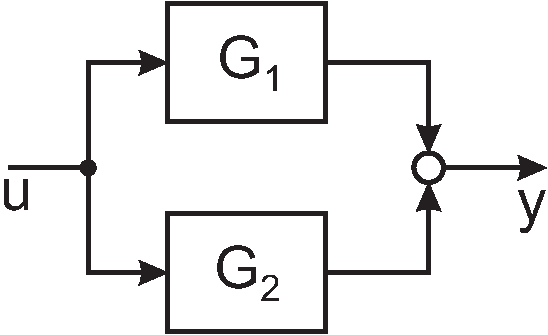
\includegraphics[width=0.5\columnwidth]{Grafiken/Parallelschaltung}
\end{center}
\begin{equation*}
G(s)=G_1(s)+G_2(s)
\end{equation*}

\subsubsection{Reihenschaltung}
\begin{center}
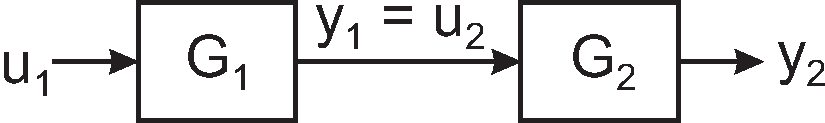
\includegraphics[width=0.8\columnwidth]{Grafiken/Reihenschaltung}
\end{center}
\begin{equation*}
G(s)=G_2(s)G_1(s)
\end{equation*}
Hier muss die Reihenfolge beachtet werden!

\subsubsection{Kreisstruktur}
\begin{center}
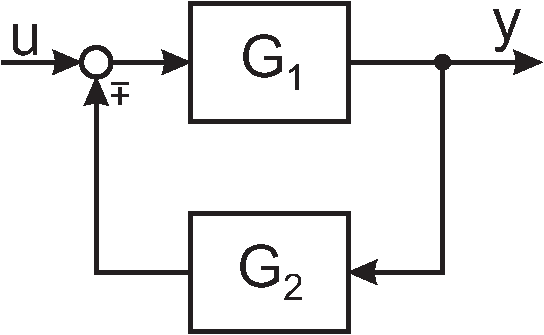
\includegraphics[width=0.5\columnwidth]{Grafiken/Kreisstruktur}
\end{center}
\begin{equation*}
\begin{split}
G(s)&=[I\pm G_1(s)G_2(s)]^{-1}G_1(s)\\
&=G_1(s)[I\pm G_2(s)G_1(s)]^{-1}
\end{split}
\end{equation*}

\subsection{Pole und Nullstellen}
\subsubsection{Pole}
Ein $p_i\in\mathbb{C}$ ist ein Pol des Systems mit Übertragungsfunktionsmatrix $G(s)$, wenn mindestens ein Element $G_{ij}(s)$ einen Pol bei $p_i$ hat.\\
Außerdem gilt:
\begin{equation*}
\begin{split}
\text{Pol}&\Leftrightarrow \text{steuer- und beobachtbarer EW von }A
\end{split}
\end{equation*}
Pole haben die folgende Bedeutung für ein LTI-System:
\begin{enumerate}[label=$\bullet$]
\item Die Pole bestimmen wesentlich die asymptotische Stabilität
\item Sie können durch Rückkopplung beeinflusst werden
\item Sie bestimmen das modale Verhalten
\item Sie beeinflussen das E/A-Verhalten
\end{enumerate}

\subsubsection{Übertragungsnullstellen (ÜNS)}
Übertragungsnullstellen eines MIMO-LTI-Systems sind Frequenzen $\mu$, für die gilt:
\begin{align*}
det(G(\mu))&=0&\text{falls }r=q\\
Rang(G(\mu))&<\max\limits_s Rang(G(s))&\text{falls }r\neq q
\end{align*}
Falls $\mu$ ein EW von $A$ ist, dann muss gelten (falls ÜNS):
\begin{enumerate}[label=$\bullet$]
\item $U\neq 0$ und endlich
\item $\lim\limits_{s\rightarrow\mu}G(s)U=0$
\end{enumerate}
\underline{\textbf{Eigenschaften:}}
\begin{enumerate}[label=$\bullet$]
\item Bei einer ÜNS verschwindet das stationäre Verhalten für eine bestimmte Frequenz
\item ÜNS sind i.A. nicht identisch mit den Nullstellen der einzelnen Matrixelemente $G_{ij}(s)$
\item ÜNS können dieselben Werte wie Pole aufweisen
\item ÜNS $\Leftrightarrow$ nicht kompensierte INS
\item Nichtquadratische Übertragungsfunktionen haben i.A. keine ÜNS, da in diesem Fall mehrere Spalten linear abhängig sein müssen, was sehr selten ist
\item Nichtsprungfähige Systeme ($D=0$) mit derselben Anzahl an Eingangs- Zustands- und Ausgangsgrößen ($n=q=r$) haben keine ÜNS\\
$\rightarrow$ Falls $B$ und $C$ quadratisch $\Rightarrow$ keine ÜNS
\item Ein System ist \textbf{minimalphasig}, wenn gilt:
\begin{equation*}
Re(\text{ÜNS})<0\;\forall\text{ ÜNS}
\end{equation*}
\end{enumerate}

\subsubsection{Invariante Nullstellen (INS)}
Als die invarianten Nullstellen eines MIMO-LTI-Systems werden diejenigen $\eta\in\mathbb{C}$ bezeichnet, für die die Rosenbrock-Systemmatrix $R(\eta)$ eine der folgenden Bedingungen erfüllt:
\begin{align*}
det(R(\eta))&=det\begin{pmatrix}\eta I-A & -B \\ C & D\end{pmatrix}=0&r=q\\
Rang(R(\eta))&<\max\limits_s Rang(R(\eta))&r\neq q
\end{align*}
\hrule
\vspace{0.2cm}
Es werden nur nicht-degenerierte und nicht-rechtssinguläre Systeme betrachtet.\\
\textbf{Degeneriert:}
\begin{align*}
Rang(R(s))<min(n+Rang(B),n+Rang(C))
\end{align*}
\textbf{Rechtssingulär:}
\begin{align*}
Rang(R(s))<n+Rang(B)
\end{align*}
Degeneriertheit $\Rightarrow$ Rechtssingularität\\
\hrule
\vspace{0.2cm}
Außerdem gilt (\textbf{Schurformel}):
\begin{equation*}
det(R(\eta))=det\begin{pmatrix}\eta I-A & -B \\ C & D\end{pmatrix}=det(\eta I-A)det(G(\eta))
\end{equation*}
Diese Formel gilt im vollen Umfang jedoch nur für $det(\eta I-A)\neq 0$. Es kann also \underline{nicht} daraus gefolgert werden, dass jeder EW eine INS ist!\\\\
\underline{\textbf{Eigenschaften:}}
\begin{enumerate}[label=$\bullet$]
\item Beschreiben inneres Verhalten
\item Anzahl INS $\geq$ Anzahl ÜNS
\item INS $\Leftrightarrow$ ENS oder ÜNS
\end{enumerate}
Eine INS ist dann eine ÜNS, wenn
\begin{enumerate}[label=$\bullet$]
\item sie mit keinem EW zusammenfällt oder
\item sie mit einem Pol zusammenfällt.
\end{enumerate}

\subsubsection{Entkopplungsnullstellen}
Eine INS $\eta$ heißt \textbf{Eingangsentkopplungsnullstelle}, wenn sie von einem nicht-steuerbaren EW von $A$ kompensiert wird bzw. wenn gilt:
\begin{equation*}
Rang\begin{pmatrix}\eta I-A & -B\end{pmatrix}<n
\end{equation*}
Eine INS $\eta$ heißt \textbf{Ausgangsentkopplungsnullstelle}, wenn sie von einem nicht-beobachtbaren EW von $A$ kompensiert wird bzw. wenn gilt:
\begin{equation*}
Rang\begin{pmatrix}\eta I-A \\ C\end{pmatrix}<n
\end{equation*}
Entkopplungsnullstellen haben die Bedeutung, dass ein nicht-steuerbarer/nicht-beobachtbarer Eigenvorgang nicht durch den Eingang angeregt werden kann oder nicht am Ausgang gemessen werden kann. Sie sind keine Übertragungsnullstellen.\\
Wenn ein System vollständig steuerbar und beobachtbar ist, gibt es keine Entkopplungsnullstellen.

\subsubsection{Überblick}
\begin{center}
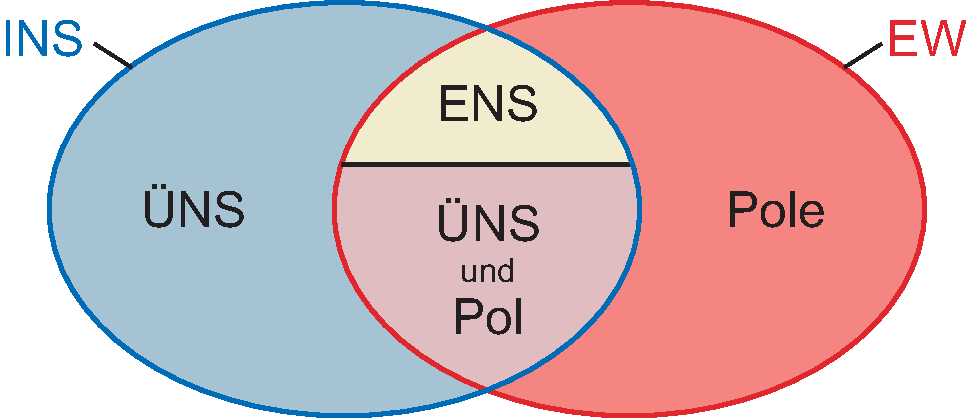
\includegraphics[width=0.8\columnwidth]{Grafiken/Pole_NS_Ueberblick}
\end{center}
\begin{align*}
\{\text{INS}\}&=\{\text{ÜNS}\}\cup\{\text{ENS}\}\\
\{\text{EW}\}&=\{\text{Pole}\}\cup\{\text{ENS}\}
\end{align*}

\subsubsection{Richtungen von Polen und Nullstellen}
Sei $s=z$ eine Nullstelle von $G(s)$ und es gibt nichttriviale Vektoren $u_z$ und $y_z^*$ (konjugiert-komplexe und transponierte Version von $y_z$), sodass
\begin{equation*}
G(z)u_z=0;\;\;y_z^*G(z)=0;\;\;\;||u_z||_2=||y_z||_2=1
\end{equation*}
$u_z$: Eingangsnullstellenrichtung\\
$y_z$: Ausgangsnullstellenrichtung\\\\
Sei außerdem $G(z)=U\Sigma V^*$ die Singulärwertzerlegung.\\\\
$\Rightarrow u_z$ ist letzte Spalte von $V$\\
$\Rightarrow y_z$ ist letzte Spalte von $U$\\\\
Für einen Pol $s=z$ gilt:
\begin{equation*}
G(p)u_p=\infty;\;\;\;y_p^*G(p)=\infty
\end{equation*}
$u_p$: Eingangspolrichtung\\
$y_p$: Ausgangspolrichtung\\\\
$\Rightarrow u_p$ ist erste Spalte von $V$\\
$\Rightarrow y_p$ ist erste Spalte von $U$

\subsubsection{Minimale und maximale Verstärkung mit Richtungen}
\begin{enumerate}
\item Berechne die EW von $G^TG$:
\begin{align*}
det(\lambda_iI-G^TG)&=0
\end{align*}
\item Berechne Verstärkungen:
\begin{align*}
\sigma_{min}&=\sqrt{\lambda_{min}}\\
\sigma_{max}&=\sqrt{\lambda_{max}}
\end{align*}
\item Berechne die dazugehörigen Richtungen $\tilde{v}_i$:
\begin{align*}
(\lambda_iI-G^TG)\tilde{v}_i=0
\end{align*}
\item Berechne die normierten Richtungen $v_i$:
\begin{align*}
v_i=\frac{1}{|\tilde{v}_i|}\cdot\tilde{v}_i
\end{align*}
\end{enumerate}

\subsubsection{Richtungsabhängigkeit der Verstärkung}
Die Verstärkung bei einem MIMO-System hängt von der Frequenz und der Richtung des Eingangs $u$ ab und ist unabhängig von der Länge des Eingangs $||u(\omega)||_2$:
\begin{equation*}
\frac{||y(\omega)||_2}{||u(\omega)||_2}=\frac{||G(j\omega)u(\omega)||_2}{||u(\omega)||_2}
\end{equation*}

\section{Steuerbarkeit und Beobachtbarkeit}
Anforderungen zur Lösbarkeit einer Regelungsaufgabe:
\begin{enumerate}
\item Steuerbarkeit und Erreichbarkeit in endlicher Zeit ($t<\infty$)
\item Stabilisierbarkeit im asymptotischen Sinn ($t\rightarrow\infty$)
\item Rekonstruierbarkeit und Beobachtbarkeit in endlicher Zeit ($t<\infty$)
\item Entdeckbarkeit im asymptotischen Sinn ($t\rightarrow\infty$)
\end{enumerate}
\underline{\textbf{Definitionen von Eingangs-Zuständen:}}
\begin{enumerate}[label=$\bullet$]
\item \textbf{Stabilisierbarkeit}:\\
Wenn für einen beliebigen Anfangszustand $x(0)=x_0$ eine Eingangsfunktion $u(t)$ existiert, sodass das System in nicht unbedingt endlicher Zeit in den Endzustand $x(t_e)=0$ gesteuert werden kann.
\item \textbf{Steuerbarkeit}:\\
Wenn für einen beliebigen Anfangszustand $x(0)=x_0$ eine Eingangsfunktion $u(t)$ existiert, sodass das System in endlicher Zeit $0<t\leq t_e<\infty$ in den Endzustand $x(t_e)=0$ gesteuert werden kann.
\item \textbf{Erreichbarkeit}:\\
Wenn für einen beliebigen Endzustand $x(t_e)=x_e$ eine Eingangsfunktion $u(t)$ existiert, in den das System in endlicher Zeit $0<t\leq t_e<\infty$ von dem Anfangszustand $x(0)=0$ aus überführt werden kann.
\end{enumerate}
\underline{\textbf{Definitionen von Ausgangs-Zuständen:}}
\begin{enumerate}[label=$\bullet$]
\item \textbf{Entdeckbarkeit}:\\
Wenn man bei gegebenem $u(t)$ aus dem zukünftigen Zeitverlauf von $y(t)$ über eine nicht unbedingt endliche Zeitspanne $t\in[0,\infty)$ den Anfangszustand $x(0)=x_0$ eindeutig ermitteln kann.
\item \textbf{Beobachtbarkeit}:\\
Wenn man bei gegebenem $u(t)$ aus dem (zukünftigen) Zeitverlauf von $y(t)$ über eine endliche Zeitspanne $t\in[0,t_e]$ den Anfangszustand $x(0)=x_0$ eindeutig ermitteln kann.
\item \textbf{Rekonstruierbarkeit}:\\
Wenn man bei gegebenem $u(t)$ aus dem (vergangenen) Zeitverlauf von $y(t)$ über eine endliche Zeitspanne $t\in[0,t_e]$ den Zustand $x(t_e)=x_e$ eindeutig rekonstruieren kann.
\end{enumerate}

\subsection{Steuerbarkeit und asymptotisches Systemverhalten}
\subsubsection{Kalman'sches Steuerbarkeitskriterium}
Das System $(A,B)$ ist genau dann steuerbar, wenn gilt:
\begin{align*}
Rang(Q_S)&=n\\
Q_S&=\left[B,AB,A^2B,...,A^{n-1}B\right]
\end{align*}

\subsubsection{Gilbert'sches Steuerbarkeitskriterium}
Das MIMO LTI-System $(\Lambda, \tilde{B})$ (in kanonischer Normalform) ist genau dann steuerbar, wenn die Matrix $\tilde{B}$ keine Nullzeile besitzt und wenn die $p$ Zeilen $\tilde{b}_i^T$, die zu den kanonischen Zustandsgrößen eines $p$-fachen Eigenwertes gehören, linear unabhängig sind.

\subsubsection{Hautus' Steuerbarkeitskriterium}
Das System $(A,B)$ ist genau dann vollständig steuerbar, wenn gilt:
\begin{equation*}
Rang(\lambda_iI-A,B)=n
\end{equation*}

\subsubsection{Stabilisierbarkeit}
Das Paar $(A,B)$ ist genau dann stabilisierbar, wenn alle $\lambda_i$ mit $Re(\lambda_i)\geq 0$ steuerbar sind:
\begin{equation*}
Rang(\lambda_i I-A,B)=n\;\;\forall\;Re(\lambda_i)\geq 0
\end{equation*}

\subsection{Beobachtbarkeit und asymptotisches Systemverhalten}
\subsubsection{Kalman'sches Beobachtbarkeitskriterium}
Das System $(A,B)$ ist genau dann beobachtbar, wenn gilt:
\begin{align*}
Rang(Q_B)&=n\\
Q_B&=\begin{bmatrix}C \\ CA \\ CA^2 \\ \vdots \\ CA^{n-1}\end{bmatrix}
\end{align*}

\subsubsection{Gilbert'sches Beobachtbarkeitskriterium}
Das System $(\Lambda,\tilde{C})$ (in kanonischer Normalform) ist genau dann beobachtbar, falls $\tilde{C}$ keine Nullspalte besitzt und wenn die $p$ Spalten $\tilde{c}_i$ von $\tilde{C}$, die zu einem $p$-fachen Eigenwert gehören, linear unabhängig sind.

\subsubsection{Hautus' Beobachtbarkeitskriterium}
Das System $(A,C)$ ist genau dann vollständig beobachtbar, wenn gilt:
\begin{equation*}
Rang\begin{pmatrix}\lambda_i I-A \\ C\end{pmatrix}=n\;\;\forall\;\lambda_i\in\lambda(A)
\end{equation*}

\subsubsection{Entdeckbarkeit}
Das Paar $(A,C)$ ist genau dann entdeckbar, wenn alle $\lambda_i$ mit $Re(\lambda_i)\geq 0$ beobachtbar sind:
\begin{equation*}
Rang\begin{pmatrix}\lambda_i I-A \\ C\end{pmatrix}=n\;\;\forall\;Re(\lambda_i)\geq 0
\end{equation*}

\section{Strukturelle Analye linearer Systeme}
\subsection{Strukturmatrizen und Strukturgraphen}
Zum Aufstellen einer Strukturmatrix müssen lediglich alle Einträge einer Matrix, die ungleich Null sind, zu 1 gesetzt werden, z.B.:
\begin{equation*}
A=\begin{pmatrix}1 & 3 & 4 \\ 0 & 5 & 4 \\ 0 & 0 & 7\end{pmatrix}\rightarrow S_A=\begin{pmatrix}1 & 1 & 1 \\ 0 & 1 & 1 \\ 0 & 0 & 1\end{pmatrix}
\end{equation*}
Anhand der Strukturmatrizen, die die Verbindungen zwischen den einzelnen Knoten $u_i, x_i,y_i$ repräsentieren, kann ein Strukturgraph erstellt werden, wie z.B.:
\begin{center}
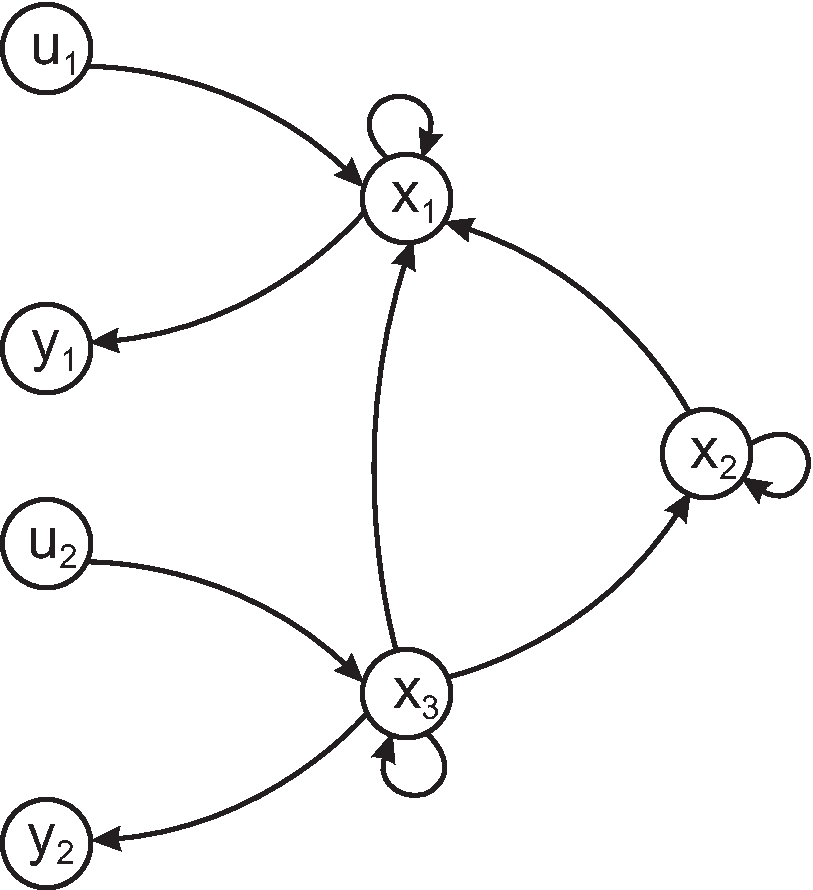
\includegraphics[width=0.6\columnwidth]{Grafiken/Strukturgraph}
\end{center}
Die Kopplungsstruktur kann mittels der Adjazenzmatrix beschrieben werden:
\begin{align*}
\begin{pmatrix}\dot{x} \\ u \\ y\end{pmatrix}=\underbrace{\begin{pmatrix}S_A & S_B & 0 \\ 0 & 0 & S_R \\ S_C & 0 & 0\end{pmatrix}}_{Ad}\cdot\begin{pmatrix}x \\ u \\ y\end{pmatrix}
\end{align*}
Falls der Ausgang nicht auf den Eingang zurückgeführt wird, gilt $S_R=0$.

\subsection{Strukturelle Steuerbarkeit und Beobachtbarkeit}
\underline{\textbf{Definitionen:}}
\begin{enumerate}[label=$\bullet$]
\item \textbf{Eingangsverbundenheit}:\\
Zu jedem Zustandsknoten $x_i$ gibt es mindestens einen Pfad, der von einem Eingangsknoten dorthin führt.
\item \textbf{Ausgangsverbundenheit}:\\
Von jedem Zustandsknoten $x_i$ gibt es einen Pfad, der zu mindestens einem Ausgangsknoten führt.
\item \textbf{Struktureller Rang ($s-Rang$)}:\\
Der strukturelle Rang einer Matrix entspricht der Anzahl an nicht-trivialen Matrixeinträgen, die so gewählt werden können, dass sie in getrennten Zeilen und Spalten stehen.
\end{enumerate}
\begin{center}
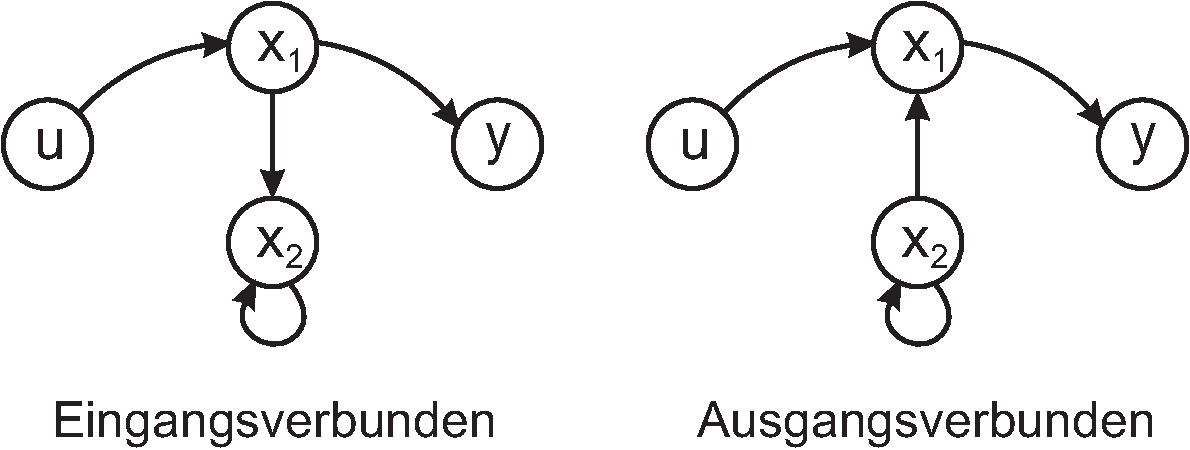
\includegraphics[width=0.9\columnwidth]{Grafiken/Ein_Ausgangsverbundenheit}
\end{center}

\subsubsection{Strukturelle Steuerbarkeit}
Eine Klasse $\mathcal{S}$ von Systemen ist strukturell steuerbar, wenn
\begin{enumerate}[label=$\bullet$]
\item $\mathcal{S}$ eingangsverbunden und
\item $s-Rang\begin{pmatrix}S_A & S_B\end{pmatrix}=n$
\end{enumerate}
Daraus folgt, dass es mindestens ein System
\begin{equation*}
\Sigma=\begin{pmatrix}A & B \\ C & 0\end{pmatrix},\Sigma\in\mathcal{S}(S_A,S_B,S_C)
\end{equation*}
gibt, das steuerbar ist.

\subsubsection{Strukturelle Beobachtbarkeit}
Eine Klasse $\mathcal{S}$ von Systemen ist strukturell beobachtbar, wenn
\begin{enumerate}[label=$\bullet$]
\item $\mathcal{S}$ ausgangsverbunden und
\item $s-Rang\begin{pmatrix}S_A \\ S_C\end{pmatrix}=n$
\end{enumerate}
Daraus folgt, dass es mindestens ein System
\begin{equation*}
\Sigma=\begin{pmatrix}A & B \\ C & 0\end{pmatrix},\Sigma\in\mathcal{S}(S_A,S_B,S_C)
\end{equation*}
gibt, das beobachtbar ist.

\subsection{Schleifenfamilie}
Unter einer \textbf{Schleifenfamilie} versteht man die Menge an geschlossenen Pfaden, die keine gemeinsamen Knoten enthalten. Zur Bestimmung der Schleifenfamilie muss eine vollständige Ausgangsrückführung hinzugefügt werden (Ausgänge mit Eingängen verbinden).\\
Die \textbf{Weite} der Schleifenfamilie gibt die Anzahl der Zustandsknoten in der Schleifenfamilie an.\\\\
\textbf{Beispiel:}\\\\
\begin{center}
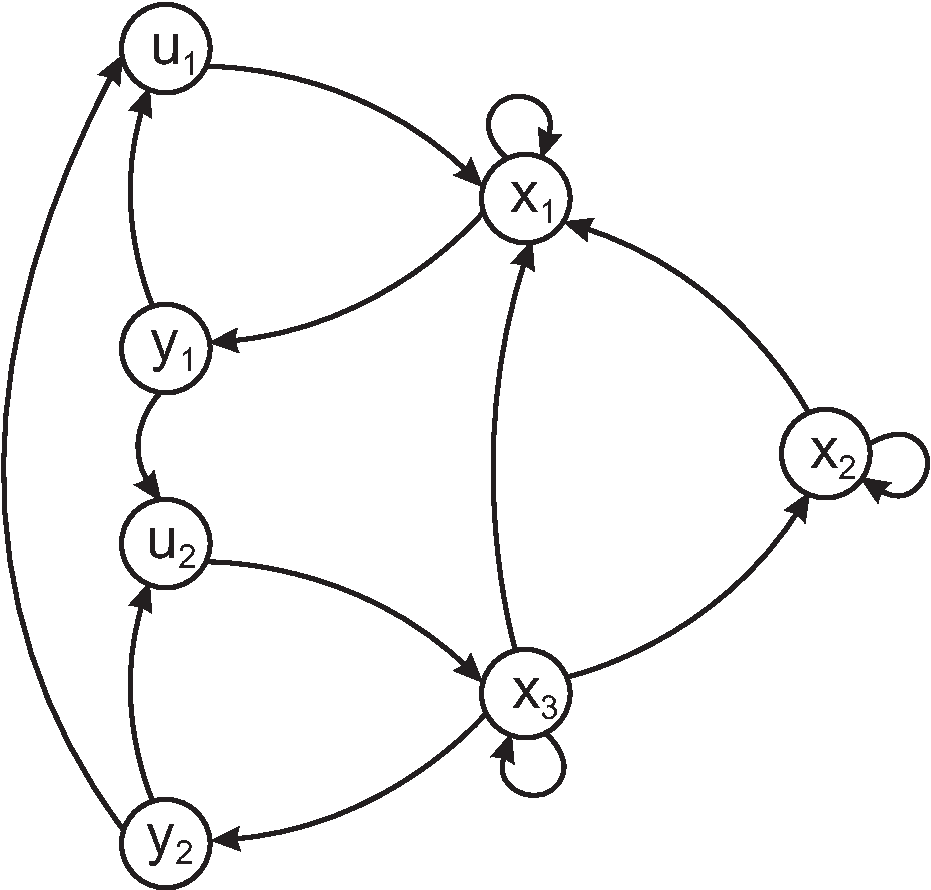
\includegraphics[width=0.7\columnwidth]{Grafiken/Schleifenfamilie}
\end{center}
1. Schleifenfamilie:\\
$\{u_2-x_3-y_2-u_2;u_1-x_1-y_1-u_1;x_2-x_2\}$\\
Weite $=n=3$\\\\
2. Schleifenfamilie:\\
$\{u_2-x_3-x_2-x_1-y_1-u_2\}$\\
Weite $=n=3$

\subsection{Strukturell feste Eigenwerte}
Strukturell feste EW sind EW, die nicht steuerbar oder nicht beobachtbar sind. Es gibt folgende zwei Typen:
\begin{enumerate}[label=$\bullet$]
\item Typ 1:\\
$\mathcal{S}$ ist entweder nicht eingangsverbunden oder nicht ausgangsverbunden oder beides.
\item Typ 2:\\
Im Strukturgraphen gibt es keine Schleifenfamilie der Weite $n$
\end{enumerate}

\section{Stabilität von MIMO-Systemen}
\underline{\textbf{Definitionen:}}
\begin{enumerate}[label=$\bullet$]
\item \textbf{Zustandsstabilität}:\\
Der Gleichgewichtszustand $x^*=0$ ist stabil, wenn es für jede beliebige Umgebung $\epsilon$ eine Umgebung um den Gleichgewichtspunkt mit dem Radius $\delta$ gibt, sodass aus $||x_0||<\delta$ die Beziehung $||x(t)||<\epsilon\;\forall\; t\geq 0$ folgt. Für asymptotische Stabilität wird zusätzlich gefordert, dass $\lim\limits_{t\rightarrow\infty}||x(t)||=0$ gilt.
\item \textbf{Ein-/Ausgangs-Stabilität}:\\
Wenn für verschwindende Anfangsauslenkungen $x_0=0$ und ein beliebiges beschränktes Eingangssignal das Ausgangssignal beschränkt bleibt.
\end{enumerate}

\subsection{Frequenzbereichsbedingungen für\\ Rückführsysteme}
\begin{center}
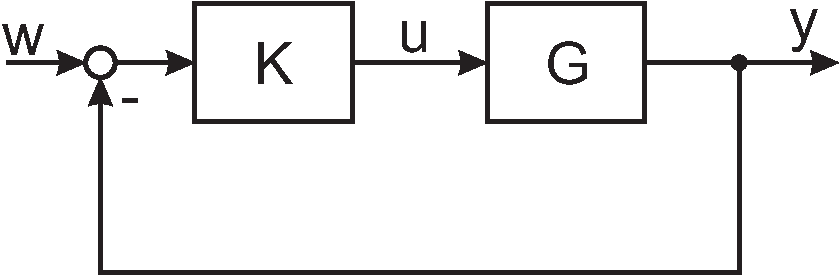
\includegraphics[width=0.8\columnwidth]{Grafiken/Rueckfuehrsysteme_Geschl_Kreis}
\end{center}
Sei
\begin{align*}
G_{ol}&=G(s)K(s)\\
F(s)&=I+G_{ol}=I+G(s)K(s)
\end{align*}
Für den dargestellten geschlossenen Kreis gilt dann:
\begin{align*}
G_w(s)&=G(s)K(s)(I+G(s)K(s))^{-1}=G_{ol}F^{-1}(s)\\
F^{-1}(s)&=\frac{1}{det(F(s))}adj(F(s))
\end{align*}
wobei $adj$ die Adjunkte der Matrix ist, also die Transponierte jener Matrix, deren Einträge die Unterdeterminanten sind.\\\\
Der Regelkreis ist genau dann E/A-stabil, wenn für die Pole $\overline{s}_i$ des geschlossenen Kreises gilt:
\begin{align*}
det(I+G(s)K(s))=0;\;\;\;Re(\overline{s}_i)<0\;\forall\;i\in\{1,...,n\}
\end{align*}

\subsubsection{Hsu-Chen-Theorem}
Wenn das System vollständig steuerbar und beobachtbar ist und der geschlossene und der offene Kreis keine gemeinsamen EW haben, dann kann die Determinante der Rückführdifferenzmatrix $F(s)$ in Abhängigkeit der Pole $\overline{s}_i$ des geschlossenen Kreises und den Polen $s_i$ des offenen Kreises geschrieben werden:
\begin{align*}
det(F(s))=k\cdot\frac{\prod\limits_{i=1}^n(s-\overline{s}_i)}{\prod\limits_{i=1}^n(s-s_i)}
\end{align*}
Unter Annahme vollständiger Beobachtbarkeit und Steuerbarkeit können somit die EW des geschlossenen und des offenen Kreises aus $F(s)$ berechnet werden.

\subsubsection{Nyquistkriterium (MIMO-Fall)}
\textbf{Voraussetzung:}
\begin{enumerate}[label=$\bullet$]
\item Der offene Kreis ist nicht sprungfähig ($D_{ol}=0$)
\end{enumerate}
Der offene Kreis mit der Übertragungsfunktionsmatrix $G_{ol}(s)$ führt genau dann auf einen (E/A-)stabilen geschlossenen Regelkreis, wenn
\begin{align*}
&\Delta arg_{\text{soll}}(det(F(j\omega)))=\left(n^++\frac{n^0}{2}\right)\pi\\
&\Delta arg(det(F(j\omega)))=\lim\limits_{\omega\rightarrow\infty}arg(det(F(j\omega)))
\end{align*}
für $\omega$ von $0$ bis $\infty$ gilt.\\\\
$n^+$: Anzahl der Pole von $G_{ol}(s)$ mit $Re(s_i)>0$\\
$n^0$: Anzahl der Pole von $G_{ol}(s)$ mit $Re(s_i)=0$\\
(mehrfache Pole zählen mehrfach!)\\\\
Wenn der offene Kreis stabil ist ($n^+=n^0=0$) und die Nyquistkurve $det(F(j\omega))$ den Ursprung der komplexen Ebene nicht umschließt, dann ist der geschlossene Regelkreis stabil.\\\\
Im Unterschied zum Nyquistkriterium für einschleifige Regelkreise liegt der kritische Punkt jetzt nicht mehr bei $-1$, sondern im Ursprung der komplexen Ebene.\\\\
Das Nyquistkriterium kann auch anhand der EW der Matrix $F(s)$ ausgedrückt werden:\\
Ein stabiler offener Kreis führt genau dann auf einen stabilen Regelkreis, wenn die EW $\lambda_{F_i}(s)$ der Matrix $F(s)$ den Ursprung der komplexen Ebene insgesamt nicht umschlingen:
\begin{align*}
\sum\limits_{i=1}^r\Delta arg(\lambda_{F_i}(s))=0
\end{align*}

\subsubsection{Bedingung des spektralen Radius}
Sei $G_{ol}(s)$ nicht sprungfähig und E/A-stabil. Wenn
\begin{align*}
\rho(G_{ol}(j\omega))<1\;\forall\;\omega
\end{align*}
dann ist der geschlossene Kreis E/A-stabil.\\
Diese Bedingung ist nur hinreichend und nicht notwendig für die Stabilität.\\\\
Der Spektralradius ist der betragsmäßig größte EW.

\subsubsection{Small gain Theorem}
Sei $G_{ol}(s)$ nicht sprungfähig und E/A-stabil. Wenn
\begin{align*}
||G_{ol}(j\omega)||<1\;\forall\;\omega
\end{align*}
dann ist der geschlossene Regelkreis E/A-stabil.\\
Dabei ist $||.||$ eine beliebige Matrix-Norm.

\subsubsection{Gershgorintheorem}
Sei $A$ eine komplexe Matrix und sei $D_i$ die Summe der nicht-diagonal-Einträge der $i$-ten Zeile. Dann gilt für jeden EW $\lambda$ der Matrix $A$, dass es mindestens einen Index $i$ gibt, sodass
\begin{align*}
|\lambda-a_{ii}|\leq D_i
\end{align*}
Dieser Sachverhalt ist auch auf die Spaltenelemente anwendbar.\\\\
Geometrisch interpretiert beschreibt die Ungleichung Kreisflächen, die sogenannten Gershgorinkreise, mit Mittelpunkten $a_{ii}$ und Radius $D_i$. Das Theorem besagt also, dass alle $n$ EW innerhalb der $n$ Kreise liegen.
\begin{center}
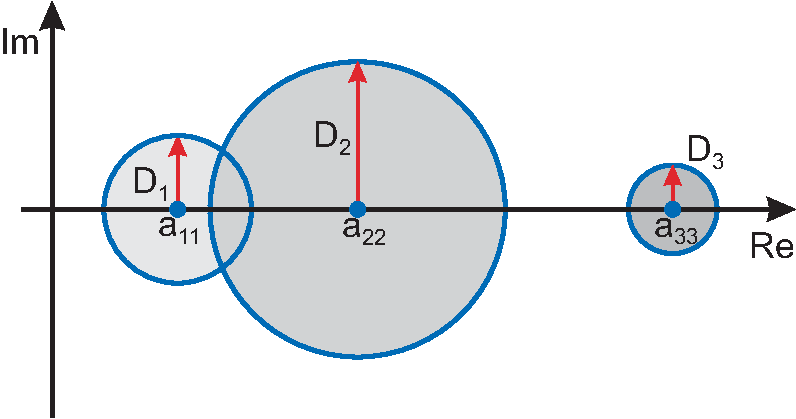
\includegraphics[width=0.95\columnwidth]{Grafiken/Gershgorintheorem}
\end{center}
\underline{\textbf{Diagonaldominanz:}}\\
Die $r\times r$ Rückführdifferenzmatrix $F(s)$ heißt \textbf{zeilendominant}, wenn
\begin{align*}
|F_{ii}(s)|>\sum\limits_{j=1,j\neq i}^r|F_{ij}(s)|\;\;\;s\in\mathcal{D}
\end{align*}
und sie heißt \textbf{spaltendominant}, wenn
\begin{align*}
|F_{ii}(s)|>\sum\limits_{j=1,j\neq i}^r|F_{ji}(s)|\;\;\;s\in\mathcal{D}
\end{align*}
Ist die Matrix entweder zeilen- oder spaltendominant, so wird sie als \textbf{diagonaldominant} bezeichnet.\\\\
Sei $G_{ol}$ stabil. Wenn $F(s)$ diagonaldominant ist und für die Hauptdiagonalelemente $F_{ii}(s)$ jeweils das SISO-Nyquistkriterium erfüllt ist, dann ist der geschlossene Kreis stabil.

\subsection{Interne Stabilität von Rückführsystemen}
\begin{center}
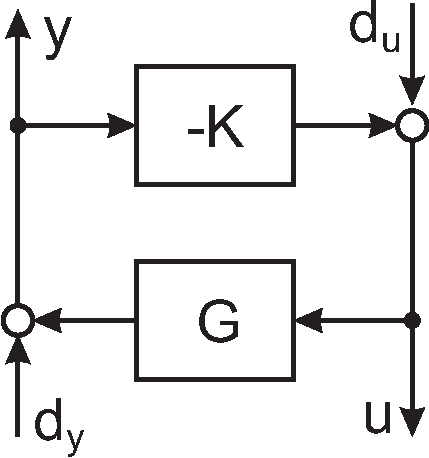
\includegraphics[width=0.5\columnwidth]{Grafiken/Rueckfuehrsystem_Stab}
\end{center}
\begin{align*}
u&=(I+KG)^{-1}d_u-K(I+GK)^{-1}d_y\\
y&=G(I+KG)^{-1}d_u+(I+GK)^{-1}d_y
\end{align*}
Das Rückführsystem ist genau dann intern stabil, wenn alle vier Übertragungsfunktionsmatrizen stabil sind.\\\\
Angenommen, es gibt keine Pol-NS-Kürzungen in der RHE zwischen $G(s)$ und $K(s)$, dann ist das Rückführsystem genau dann intern stabil, wenn eine der vier Übertragungsfunktionen stabil ist.

\subsection{Lyapunov-Stabilität und Quadratische Stabilität}
Sei
\begin{align*}
\dot{x}=Ax;\;\;\;x(0)=x_0
\end{align*}

\subsubsection{Lyapunov-Stabilität}
Ein Gleichgewichtspunkt $x^*$ eines autonomen Systems heißt
\begin{enumerate}[label=$\bullet$]
\item \textbf{stabil}, wenn es zu jedem gegebenen $\epsilon>0$ ein $\delta(\epsilon)>0$ gibt, sodass
\begin{align*}
||x_0-x^*||<\delta(\epsilon)\Rightarrow ||x(t)-x^*||<\epsilon\;\forall\;t\geq 0
\end{align*}
\item \textbf{asymptotisch stabil}, wenn er stabil und attraktiv ist, sodass
\begin{align*}
||x_0-x^*||<\delta\Rightarrow \lim\limits_{t\rightarrow\infty}||x(t)-x^*||=0
\end{align*}
\end{enumerate}

\subsubsection{Direkte Methode von Lyapunov}
Sei $x^*\in X$ eine Ruhelage des Systems $\dot{x}=f(x),x(0)=x_0$.
Die Ruhelage ist
\begin{enumerate}[label=$\bullet$]
\item \textbf{stabil}, falls folgende Eigenschaften gelten:
\begin{enumerate}
\item $V(x^*)=0$
\item $V(x)>0$ für alle $x\neq x^*$
\item $\dot{V}=\frac{d}{dt}V(x)\leq 0$
\end{enumerate}
\item \textbf{asymptotisch stabil}, falls sie stabil ist und $\dot{V}(x)< 0$.
\end{enumerate}

\subsubsection{Quadratische Stabilität}
Das LTI-System mit $x^*=0$ heißt quadratisch stabil, wenn es asymptotisch stabil ist im Sinne von Lyapunov, wobei die Lyapunovfunktion folgende Form besitzt:
\begin{align*}
V(x)=x^TPx;\;\;\;P=P^T\succ 0
\end{align*}
Ein LTI-System ist genau dann zustandsstabil, wenn es quadratisch stabil ist.\\\\
Seien $P$ und $Q$ symmetrische, positiv definite Matrizen, dann muss gelten:
\begin{equation*}
A^TP+PA=-Q
\end{equation*}
Vorgehensweise, um asymptotische Stabilität nachzuweisen:
\begin{enumerate}
\item Wähle $Q$ als symmetrische, positiv definite Matrix (z.B. $Q=I_n$)
\item Einsetzen von allgemeinem symmetrischen Ansatz für $P$:
\begin{equation*}
P=\begin{bmatrix}p_1 & p_2 & ... \\ p_2 & p_3 & \vdots \\ \vdots & ... & \ddots\end{bmatrix}
\end{equation*}
\item
\begin{enumerate}[label=$\bullet$]
\item Falls $P$ nicht positiv definit\\
$\Rightarrow$ System nicht asymptotisch stabil
\item Falls $P$ positiv definit\\
$\Rightarrow$ System asymptotisch stabil
\end{enumerate}
\end{enumerate}
Eine symmetrische Matrix ist positiv definit, falls gilt:
\begin{equation*}
\lambda_i>0\;\;\forall i
\end{equation*}

\section{Reglerentwurfsverfahren}
Allgemeines Regelgesetz für LTI-Systeme:
\begin{align*}
u(t)&=-Kx(t)+Lw(t);\;\;\;K\in\mathbb{R}^{r\times n};L\in\mathbb{R}^{r\times q}\\
\Rightarrow\dot{x}&=(A-BK)x+BLw\\
y&=Cx
\end{align*}
\textbf{Anforderungen:}
\begin{enumerate}[label=$\bullet$]
\item Reglerstabilität (Rückführmatrix $K$):
\begin{align*}
x(t)\rightarrow 0,\;\;\text{für }t\rightarrow\infty\text{ mit }w=0
\end{align*}
\item Stationäre Genauigkeit (Vorfiltermatrix $L$):
\begin{align*}
y(t)\rightarrow w,\;\;\;\text{für }t\rightarrow\infty\text{ mit }w=\text{const.}
\end{align*}
\end{enumerate}
\begin{center}
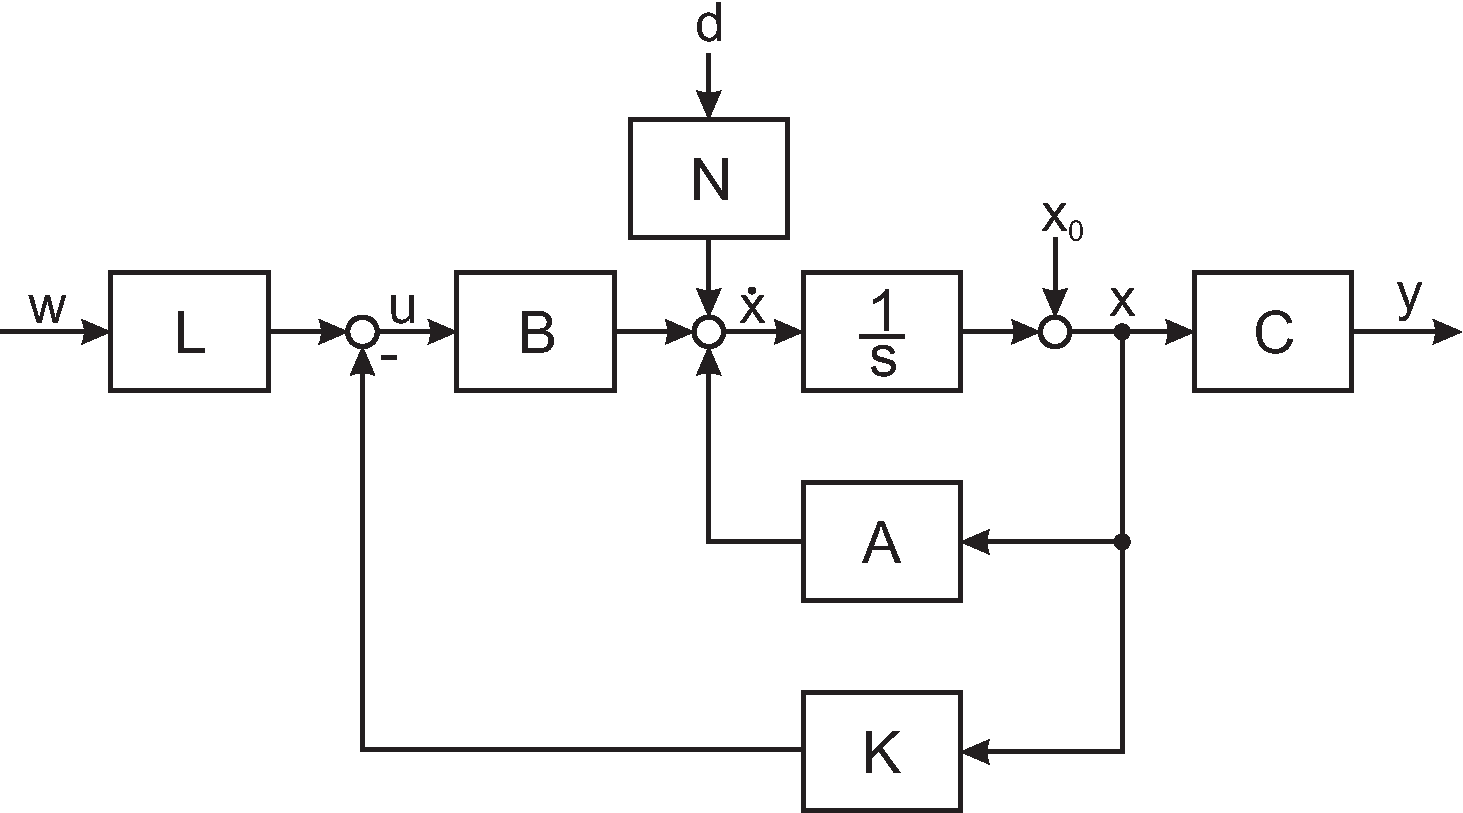
\includegraphics[width=0.98\columnwidth]{Grafiken/Struktur_Zustandsregelung}
\end{center}

\subsection{Wahl der Vorfiltermatrix $L$}
Um stationäre Genauigkeit zu erreichen, muss gelten:
\begin{align*}
\dot{x}&=0\\
\Leftrightarrow L&=\left[C(BK-A)^{-1}B\right]^{-1}\;\;\;(\text{für }q=r)
\end{align*}
Die benötigten Inversen existieren, wenn gilt:
\begin{enumerate}
\item System asymptotisch stabil:
\begin{align*}
Re\{\lambda(A-BK)\}<0\;\;\forall\;\lambda(A-BK)
\end{align*}
\item Es gibt keine invariante Nullstelle $\eta_i$ in Null:\\
(Die INS des geregelten Systems entsprechen generell genau den INS des ungeregelten Systems)
\begin{align*}
det(R_K(\eta))&=det\begin{pmatrix}\eta I-A & -B \\ C & 0\end{pmatrix}=0
\end{align*}
\end{enumerate}
Diese Vorgehensweise ist allerdings nur anwendbar, wenn sich der Führungsvektor $w$ im Vergleich zur Regelkreisdynamik relativ langsam ändert; Ansonsten ist die Entkoppelung nach Falb-Wolovich notwendig.

\subsection{Vollständige Modale Synthese nach Roppenecker}
Die Rückführmatrix $K$ zur Polvorgabe nach Roppenecker ergibt sich über
\begin{align*}
K&=(p_1,...,p_n)\left[(A-\lambda_{K1}I)^{-1}Bp_1,...,(A-\lambda_{Kn}I)^{-1}Bp_n\right]^{-1}\\
&=(p_1,...,p_n)(v_{K1},...,v_{Kn})^{-1}
\end{align*}
mit
\begin{align*}
v_{Ki}&=(A-\lambda_{Ki}I)^{-1}Bp_i\\
(A-\lambda_{Ki}I)v_{Ki}&=Bp_i
\end{align*}
\begin{tabular}{ll}
$\lambda_{Ki}$: & Gewünschte Regelungseigenwerte von $A-BK$\\
$p_i$: & Parametervektoren (beliebig wählbar)\\
$v_{Ki}$: & Eigenvektoren von $A-BK$
\end{tabular}\\\\\\
\textbf{Voraussetzungen:}
\begin{enumerate}[label=$\bullet$]
\item $B$ hat vollen Rang und
\item EV $v_{Ki}$ sind linear unabhängig (z.B. wenn die EW $\lambda_{Ki}$ einfach und von den Strecken-EW $\lambda_i$ verschieden sind).
\end{enumerate}
\textbf{Vorgehensweise:}
\begin{enumerate}
\item Regelungs-EV $v_{Ki}$ aus $\lambda_{Ki}$ und $p_i$ berechnen.
\item Reglermatrix $K$ bestimmen.
\item Vorfiltermatrix $L$ bestimmen.
\end{enumerate}
Durch gezielte Wahl der Parametervektoren $p_i$ können bestimmte Anforderungen erfüllt werden, wie z.B.:
\begin{enumerate}[label=$\bullet$]
\item Spalten von $K$ zu Null machen: dadurch kann auf Messung der betreffenden Zustandsgröße verzichtet werden.
\item Einzelne Elemente von $K$ zu Null machen: dezentrale Zustandsrückführung
\item Stellgrößenausschläge verringern.
\item Robustheit erhöhen.
\item Soll ein Strecken-EW erhalten bleiben, so setzt man $v_{Kj}=v_j$ und $p_j=0$.
\end{enumerate}

\subsection{Regelung für Störentkoppelung}
Betrachtet wird folgendes System:
\begin{align*}
\dot{x}&=Ax+Bu+Nd,\;\;\;x_0=0\\
y&=Cx\\
u&=-Kx
\end{align*}
\begin{tabular}{ll}
$d:$ & Störgrößenvektor\\
$N:$ & Störungsabbildungsmatrix
\end{tabular}\\\\\\
Das Störentkoppelungsproblem besteht darin, einen Zustandsregler $u=-Kx$ so zu finden, dass für alle Zeiten $t>0$ die Störung $d(t)$ nicht auf den Ausgang $y(t)$ wirkt.
\begin{align*}
\Rightarrow&\text{Abbildung der Störung auf einen nicht beobachtbaren}\\
&\text{Unterraum.}
\end{align*}
Dies ist der Fall, wenn sich die Spaltenvektoren von $N$ über nicht-beobachtbare Basisvektoren darstellen lassen. Dafür muss gelten:
\begin{align*}
\underbrace{\begin{bmatrix}\lambda_{Ki}I-A & B \\ C & 0\end{bmatrix}}_{R(\lambda_{Ki})}\begin{bmatrix}v_{Ki} \\ p_i\end{bmatrix}&=0\\
\Rightarrow det(R(\lambda_{Ki}))=det\begin{pmatrix}\lambda_{Ki}I-A & B \\ C & 0\end{pmatrix}&=0
\end{align*}
Regelungs-EW entsprechen INS ($\lambda_{Ki}=\eta_i$).\\\\
\textbf{Bestimmung einer vollständigen Zustandsrückführung mit Störentkopplung:}
\begin{enumerate}
\item Bestimme linear unabhängige $v_{Ki}$ mit
\begin{align*}
Cv_{Ki}=0
\end{align*}
Wenn die $v_{Ki}$ keine Basis von $N$ bilden, dann ist eine Störentkoppelung nicht möglich.
\item Bestimme $k$ (Anzahl der $v_{Ki}$) INS $\eta_i=\lambda_{Ki}$:
\begin{align*}
det\begin{pmatrix}\lambda_{Ki}I-A & B \\ C & 0\end{pmatrix}=0
\end{align*}
und berechne danach die zugehörigen $p_i$:
\begin{align*}
(\lambda_{Ki}I-A)v_{Ki}=-Bp_i
\end{align*}
\item Die restlichen $n-k$ EW mit Parametervektoren sind frei wählbar
\item Berechne die EV der restlichen EW:
\begin{align*}
(\lambda_iI-A)v_{Ki}=0
\end{align*}
\item Berechne $K$:
\begin{align*}
K=(p_1,...,p_n)(v_1,...,v_n)^{-1}
\end{align*}
\item Evtl. Test, ob $G_d=0$:
\begin{align*}
G_d=C(sI-(\underbrace{A-BK}_{A_k}))^{-1}N
\end{align*}
\end{enumerate}

\subsection{Entkopplungsregelung nach Falb-Wolovich}
Betrachtet wird folgendes System:
\begin{align*}
\dot{x}&=Ax+Bu\\
y&=Cx\\
u&=-Kx+Lw
\end{align*}
Ziel der Entkoppelungsregelung ist es, $K$ und $L$ so zu wählen, dass das System entkoppelt wird, d.h. damit aus dem MIMO-System $q$ SISO-Systeme werden ($q=r$).\\\\
\textbf{Definition:}
\begin{enumerate}[label=$\bullet$]
\item Ein MIMO-LTI-System hat die \textbf{Differenzenordnung} bzw. \textbf{den relativen Grad} $(\delta_1,...,\delta_q)$, wenn für $i=1,...,q$ gilt:
\begin{align*}
c_i^TA^jB&=0\;\;\;\forall j=0,...,\delta_i-2\\
c_i^TA^{\delta_i-1}B&\neq 0
\end{align*}
wobei $c_i^T$ die $i$-te Zeile von $C$ darstellt.
\item Alternative Bestimmungsmethode:\\
Leite $y_i$ so oft ab ($\delta_i$-mal), bis $y_i^{(\delta_i)}$ direkt von $u$ abhängt.
\item Die \textbf{Gesamtdifferenzenordnung} ist
\begin{align*}
\delta =\sum\limits_i \delta_i
\end{align*}
\end{enumerate}
\textbf{Vorgehensweise:}
\begin{enumerate}
\item Bestimme $\delta$ und mache Fallunterscheidung:
\begin{enumerate}[label=$\bullet$]
\item $\delta=n$: weiter mit 2.
\item $\delta<n$: es existieren Entkopplungsnullstellen, die stabil sein müssen. Falls $Re(\eta)>0$, dann ist eine Entkoppelungsregelung instabil.
\end{enumerate}
\item Berechne $E$:
\begin{align*}
E=\begin{bmatrix}c_1^TA^{(\delta_1-1)}B \\ \vdots \\ c_q^TA^{(\delta_q-1)}B\end{bmatrix}
\end{align*}
Falls $det(E)\neq 0$, dann weiter mit 3.
\item Vorfilter $L$ berechnen:
\begin{align*}
L&=E^{-1}T\\
T&=\begin{bmatrix}\gamma_i & ... & 0 \\ \vdots & \ddots & \vdots \\ 0 & ... & \gamma_q\end{bmatrix}
\end{align*}
Mit den vorgegebenen Übertragungsfunktionen können dann die $\gamma_i$ und $M_{ij}$ berechnet werden:
\begin{align*}
\left(\frac{y_i(s)}{w_i(s)}\right)_{soll}&=\frac{\gamma_i}{s^{\delta_i}+...+M_{i1}s+M_{i0}}
\end{align*}
\item Reglermatrix $K$ berechnen:
\begin{align*}
K=E^{-1}\begin{bmatrix}c_1^TA^{\delta_1}+\sum\limits_{j=0}^{\delta_1-1}M_{1j}c_1^TA^j \\ \vdots \\ c_q^TA^{\delta_q}+\sum\limits_{j=0}^{\delta_q-1}M_{qj}c_q^TA^j\end{bmatrix}
\end{align*}
\end{enumerate}

\subsection{Direktes Nyquistkriterium zum Entwurf dezentraler Regler}
Betrachtet wird das System:
\begin{align*}
\dot{x}&=Ax+Bu\\
y&=Cx
\end{align*}
Bei der dezentralen Regelung werden die Vektoren in Teilvektoren zerlegt, die aus $N$ Teilsystemen bestehen.
\begin{align*}
\begin{pmatrix}\dot{x}_1 \\ \vdots \\ \dot{x}_N\end{pmatrix}&=\begin{pmatrix}A_1 & & 0 \\ & \ddots & \\ 0 & & A_N\end{pmatrix}\begin{pmatrix}x_1 \\ \vdots \\ x_N\end{pmatrix}+\begin{pmatrix}B_1 & & 0 \\ & \ddots & \\ 0 & & B_N\end{pmatrix}\begin{pmatrix}u_1 \\ \vdots \\ u_N\end{pmatrix}\\
\begin{pmatrix}y_1 \\ \vdots \\ y_N\end{pmatrix}&=\begin{pmatrix}C_1 & & 0 \\ & \ddots & \\ 0 & & C_N\end{pmatrix}\begin{pmatrix}x_1 \\ \vdots \\ x_N\end{pmatrix}\\
\begin{pmatrix}u_1 \\ \vdots \\ u_N\end{pmatrix}&=-\begin{pmatrix}K_1 & & 0 \\ & \ddots & \\ 0 & & K_N\end{pmatrix}\begin{pmatrix}x_1 \\ \vdots \\ x_N\end{pmatrix}
\end{align*}
Das Problem ist es, die Auswirkung der durch Vernachlässigung der Querkopplungen entstehenden Störung richtig zu beurteilen.
\begin{center}
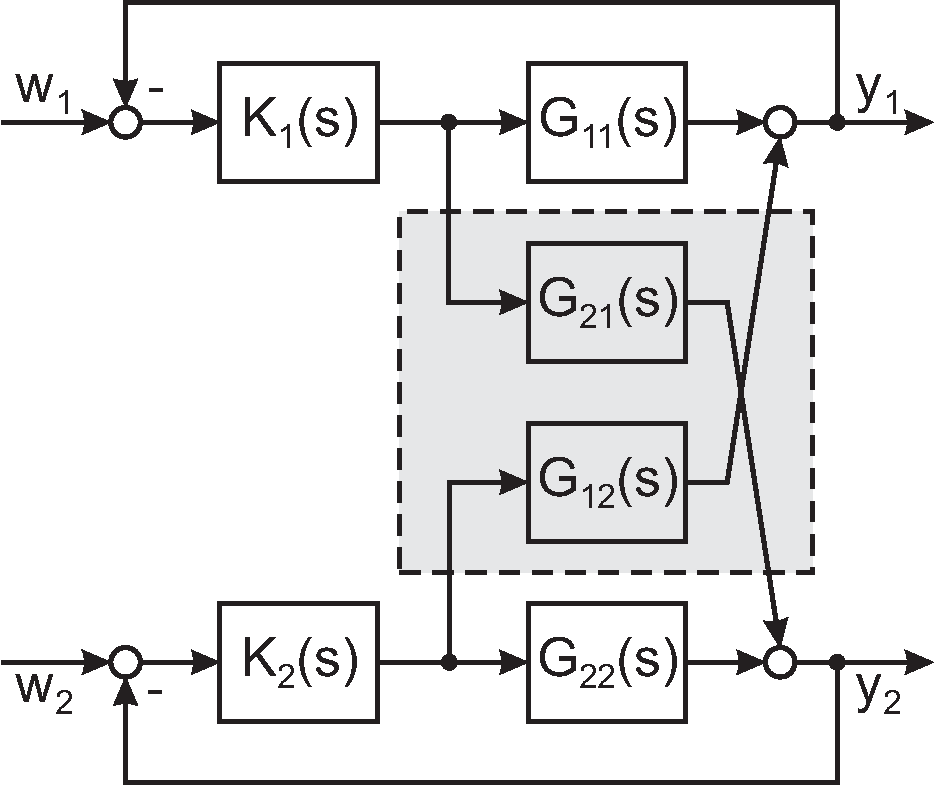
\includegraphics[width=0.9\columnwidth]{Grafiken/Dezentraler_Regler_Querkopplungen}
\end{center}
Der aus $r$ Eingrößenreglern $K_i(s),i=1,...,r$ und der Regelstrecke $G(s)$ bestehende \textbf{Regelkreis ist stabil, falls}
\begin{enumerate}[label=$\bullet$]
\item die ÜF $G_{oli}(s),i=1,...,r$ der offenen Ketten der Eingrößenregelkreise den Punkt $-1$ insgesamt $n^+$-Mal gegen den Uhrzeigersinn umschlingen.\\
($n^+$: Anzahl der Pole mit positivem Realteil)
\item $F(s)=I+G_{ol}(s)$ diagonaldominant ist.
\end{enumerate}

\subsubsection{Direktes Nyquistverfahren zum Entwurf dezentraler Regeleinrichtungen}
\textbf{Voraussetzungen:}
\begin{enumerate}[label=$\bullet$]
\item $D=0$, d.h. das System ist nicht sprungfähig
\item $G$ ist näherungsweise diagonaldominant
\item Die Regelstrecke ist E/A-stabil
\end{enumerate}
\textbf{Entwurf eines dezentralen Reglers:}
\begin{enumerate}
\item Entwurf von $r$ Eingrößenreglern $K_i(s)$ für die $G_{ii}(s)$.
\item Überprüfen der Diagonaldominanz von $F(s)$. Wenn dies nicht vorliegt, muss durch geeignete Wahl anderer Eingrößenregler versucht werden, Diagonaldominanz herzustellen.
\item Untersuchen der Regelgüte des dezentral geregelten Systems anhand von Simulationen.
\end{enumerate}

\subsection{Relative Gain Array (RGA)}
Das RGA ist ein Maß für Interaktion in der Form von Kopplung in MIMO-Systemen. Je näher es an der Identität $I$ ist, desto geringer ist die Interaktion.
\begin{align*}
RGA(G)=G\times(G^{-1})^T
\end{align*}
wobei $\times$ elementweise Multiplikation bedeutet.

\section{Grundlagen Performanzorientierter Regelung von MIMO-LTI-Systemen}
\subsection{Grundlegende Definitionen}
Betrachtet werden geschlossene Regelkreise unter Störeinfluss $d$ und Messrauschen $n$:
\begin{center}
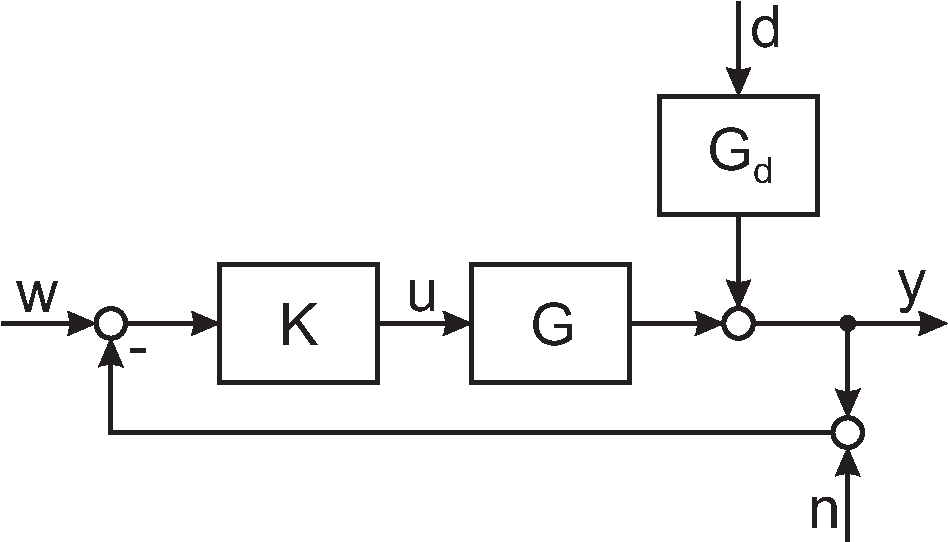
\includegraphics[width=0.8\columnwidth]{Grafiken/Blockdiagramm_Regelungssystem}
\end{center}
Es gilt:
\begin{align*}
y&=\underbrace{(I+GK)^{-1}GK}_{=G_w}w+\underbrace{(I+GK)^{-1}}_{=F^{-1}}G_dd-\underbrace{(I+GK)^{-1}GK}_{=G_w}n\\
&=Tw+SG_dd-Tn
\end{align*}
\textbf{Definintionen:}
\begin{enumerate}[label=$\bullet$]
\item \textbf{Sensitivitätsfunktionsmatrix} $S$ und \textbf{komplementäre Sensitivitätsfunktionsmatrix} $T$:
\begin{align*}
S&=(I+GK)^{-1}=(I+G_{ol})^{-1}\\
T&=(I+GK)^{-1}GK=(I+G_{ol})^{-1}G_{ol}\\
\Rightarrow S+T&=I
\end{align*}
\end{enumerate}
Außerdem gilt:
\begin{align*}
u&=K(w-y-n)=KS(w-G_dd-n)\\
e&=w-y=S(w-G_dd)+Tn
\end{align*}
Die Regelabweichung in Bezug zur Führungsgröße ist somit:
\begin{align*}
e=Sw
\end{align*}
\textbf{Definitionen:}
\begin{enumerate}[label=$\bullet$]
\item Sei $\omega_1=0$ im Intervall $[\omega_1,\omega_2]$.\\
Die \textbf{(Sensitivitäts-)Bandbreite} (des geschlossenen Kreises) ist die Frequenz $\omega_B=\omega_2$, bei der der Amplitudenverlauf $|S(j\omega)|$ zum ersten Mal $\frac{1}{\sqrt{2}}=0.707\;(\approx 3dB)$ von unten schneidet.
\item Die \textbf{Bandbreite mit Bezug auf $T$}, bezeichnet als $\omega_{BT}$, ist die höchste Frequenz, bei der der Amplitudenverlauf $|T(j\omega)|$ den Wert $\frac{1}{\sqrt{2}}=0.707\;(\approx -3dB)$ von oben schneidet.
\item Die \textbf{Durchtrittsfrequenz} $\omega_c$ ist die Frequenz, bei der der Amplitudenverlauf $|G_{ol}(j\omega)|$ zum ersten mal Eins von oben schneidet.
\item Die \textbf{Phasendurchtrittsfrequenz} $\omega_{180}$ ist die Frequenz, bei welcher die Nyquist-Kurve von $G_{ol}(j\omega)$ zum ersten mal die negative Achse zwischen -1 und 0 schneidet.
\end{enumerate}
Die Frequenzen $\omega_B,\omega_{BT}$ und $\omega_c$ nehmen oftmals ähnliche Werte an. Ist dies nicht der Fall, so ist $\omega_B$ i.d.R. von größerer Bedeutung für das Regelverhalten.\\\\
Typische Verläufe von $|S|$ und $|T|$:
\begin{center}
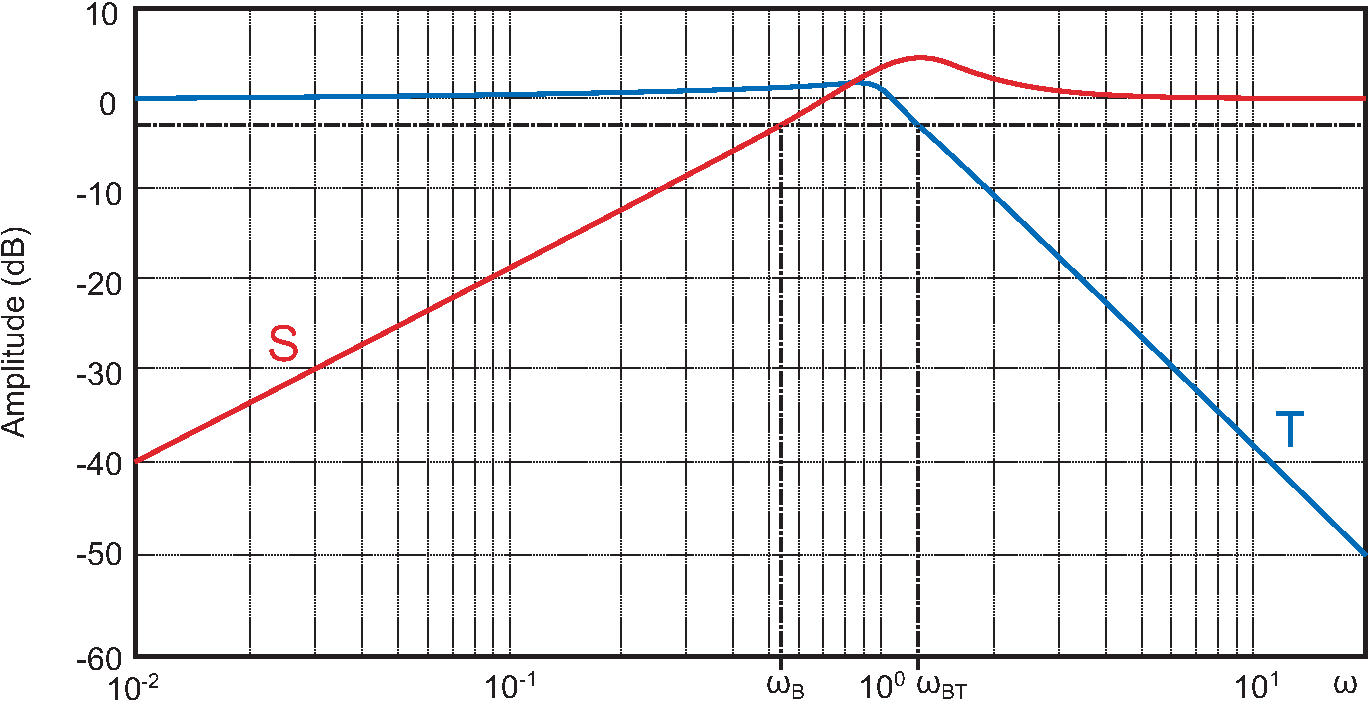
\includegraphics[width=0.98\columnwidth]{Grafiken/Bodediagramm_S_T}
\end{center}
Die Amplitudenverläufe werden im MIMO-Fall i.d.R. über den Verlauf des größten Singulärwertes der Übertragungsfunktionsmatrizen angegeben.

\subsection{Spezifikationen und Loop Shaping}
\subsubsection{Qualitative Forderungen zum Closed-Loop Shaping}
\textbf{Qualitative Ziele:}
\begin{enumerate}[label=$\bullet$]
\item \textbf{Gutes Folgeverhalten} liegt vor, wenn $y/w\rightarrow I$,d.h.:
\begin{align*}
T(j\omega)\overset{!}{\rightarrow}I
\end{align*}
Für Open-Loop Shaping gilt:\\
Amplitudenwert von $G_{ol}$ sollte möglichst groß sein.
\item \textbf{Gute Störunterdrückung} wird realisiert, wenn $y/d\rightarrow 0$ bzw.:
\begin{align*}
S(j\omega)\overset{!}{\rightarrow}0\Rightarrow|S(j\omega)|\overset{!}{\rightarrow}0
\end{align*}
Für Open-Loop Shaping gilt:\\
$|G_{ol}|$ sollte möglichst groß sein.
\item \textbf{Gute Rauschunterdrückung} wird erzielt, wenn $y/n\rightarrow 0$ bzw.:
\begin{align*}
T(j\omega)\overset{!}{\rightarrow}0\Rightarrow |T(j\omega)|\overset{!}{\rightarrow}0\text{ für hohe Frequenzen}
\end{align*}
Für Open-Loop Shaping gilt:\\
$|G_{ol}|$ sollte möglichst klein sein.
\item \textbf{Niedriger Energieaufwand} im Sinne von kleinen Stellgrößen, wenn $u/w\rightarrow 0$ bzw.:
\begin{align*}
K(j\omega)S(j\omega)\overset{!}{\rightarrow}0\Rightarrow |K(j\omega)S(j\omega)|\overset{!}{\rightarrow}0
\end{align*}
Für Open-Loop Shaping gilt:\\
$|G_{ol}|$ sollte möglichst klein sein.
\end{enumerate}

\subsubsection{Quantitative Forderungen beim Closed-Loop Shaping und Gewichtete Sensitivität}
\textbf{Quantitative Forderungen:}
\begin{enumerate}[label=$\bullet$]
\item Gewährleistung einer bestimmten Bandbreite:
\begin{align*}
|S(j\omega)|\leq -3dB,\;\;\;\forall\omega\leq \omega_B
\end{align*}
\item Beschränkung des stationären Folgefehlers $e$:
\begin{align*}
\lim\limits_{t\rightarrow\infty}|e(t)|=\lim\limits_{s\rightarrow 0}|S(s)W(s)|\overset{!}{<}A
\end{align*}
A: maximale Amplitude
\item Begrenzung des maximalen Regelfehlers:
\begin{align*}
\max\limits_{\omega}|S(j\omega)|\overset{!}{\leq}M
\end{align*}
\end{enumerate}
Eine typische obere \textbf{Schrankenfunktion} ist gegeben durch:
\begin{align*}
w_S(s)&=\frac{\frac{s}{M}+\omega_B}{s+\omega_BA}
\end{align*}
Es gilt:
\begin{align*}
\lim\limits_{\omega\rightarrow 0}\frac{1}{w_S(j\omega)}&=A&\;\;\;\;\;\;\text{(min. Verstärkung)}\\
\lim\limits_{\omega\rightarrow \infty}\frac{1}{w_S(j\omega)}&=M&\;\;\;\;\;\;\text{(max. Verstärkung)}
\end{align*}
Die Spezifikationen werden dann eingehalten, wenn gilt:
\begin{align*}
|w_S(s)S(s)|&\leq\max||w_S(s)S(s)||_2=||w_S(s)S(s)||_{\infty}<1\\
|S(j\omega)|&<\frac{1}{|w_S(j\omega)|}
\end{align*}
Bedingung an die \textbf{gewichtete Sensitivität} $w_SS$:
\begin{align*}
|w_SS|\leq|w_S||S|&\overset{!}{<}1,\;\;\;\forall\omega
\end{align*}
In gleicher Weise können auch Schrankenfunktionen für $T(w_T)$ und den Energieverbrauch $KS(w_u)$ spezifiziert werden:
\begin{align*}
||w_T(\omega)T(j\omega)||_{\infty}&<1\\
||w_u(\omega)KS(j\omega)||_{\infty}&<1
\end{align*}

\subsection{Beschränkungen der Performanz}
\subsubsection{SISO Interpolationsbeschränkung}
Unter der Annahme, dass sich in $G_{ol}=GK$ keine instabilen Pole mit Nullstellen kürzen, so gilt:
\begin{enumerate}[label=$\bullet$]
\item Wenn $p\in$ RHE Pol von $G_{ol}$ ist, dann gilt:
\begin{align*}
S(p)=0\text{ und }T(p)=1
\end{align*}
\item Wenn $z\in$ RHE Nullstelle von $G_{ol}$ ist, dann gilt:
\begin{align*}
S(z)=1\text{ und }T(z)=0
\end{align*}
\end{enumerate}

\subsubsection{MIMO Interpolationsbeschränkung}
Sei die Menge der Pole und Nullstellen von $G_{ol}$, die in der RHE liegen, disjunkt. Für $S$ und $T$ muss dann gelten:
\begin{enumerate}[label=$\bullet$]
\item Wenn $p\in$ RHE Pol von $G$ ist mit Eingangspolrichtung $u_p$, dann gilt:
\begin{align*}
S(p)u_p=0\text{ und }T(p)u_p=u_p
\end{align*}
\item Wenn $z\in$ RHE Nullstelle von $G$ ist mit Ausgangsnullstellenrichtung $y_z$, dann gilt:
\begin{align*}
y_z^*S(z)=y_z^*\text{ und }y_z^*T(z)=0^T
\end{align*}
\item Wenn $p\in$ RHE Pol von $K$ ist mit Ausgangspolrichtung $y_{p,K}$, dann gilt:
\begin{align*}
y_{p,K}^*S(p)=0^T\text{ und }y_p^*T(p)=y_{p,K}^*
\end{align*}
\item Wenn $z\in$ RHE Nullstelle von $K$ ist mit Eingangsnullstellenrichtung $u_{z,K}$, dann gilt:
\begin{align*}
S(z)u_{z,k}=u_{z,k}\text{ und }T(z)u_{z,k}=0
\end{align*}
\end{enumerate}

\subsubsection{Bode-Sensitivitätsintegral und Wasserbetteffekt (SISO-Fall)}
Sei $\{p_i:i=1,...,n_p\}$ die Menge der Pole von $G_{ol}$ in der RHE, $G_{ol}$ ist rational mit relativem Grad $\delta\geq 1$. Wenn der geschlossene Regelkreis stabil ist, dann gilt für
\begin{enumerate}[label=$\bullet$]
\item $G_{ol}$ proper mit $\delta=1$, dass
\begin{align*}
\int\limits_0^{\infty}log|S(j\omega)|d\omega=-\frac{\pi}{2}\lim\limits_{s\rightarrow\infty}sG_{ol}+\pi\sum\limits_{i=1}^{n_p}Re(p_i)
\end{align*}
\item $G_{ol}=G_{ol,0}e^{-s\tau},\;\tau>0$, $G_{ol,0}$ streng proper (bzw. $\delta>1$), dass
\begin{align*}
\int\limits_0^{\infty}log|S(j\omega)|d\omega=\pi\sum\limits_{i=1}^{n_p}Re(p_i)
\end{align*}
\end{enumerate}

\subsubsection{Poisson-Sensitivitätsintegrale und Sensitivitätspeaks (SISO-Fall)}
\textbf{Blaschke-Produkt} der NS und Pole in der RHE:
\begin{align*}
B_S(s)=\prod\limits_{i=1}^{n_p}\frac{p_i-s}{p_i^*+s}\text{ und }B_T(s)=\prod\limits_{i=1}^{n_z}\frac{z_i-s}{z_i^*+s}
\end{align*}
Diese Blaschke-Produkte sind Allpassfunktionen.\\
Es ergibt sich:
\begin{align*}
G_{ol}(s)&=\tilde{G}_{ol}(s)B_S^{-1}(s)B_T(s)e^{-s\tau},\;\;\;\tau >0\\
S(s)&=\tilde{S}(s)B_S(s)\\
T(s)&=\tilde{T}(s)B_T(s)e^{-s\tau}
\end{align*}
Sei der offene Kreis $G_{ol}$ faktorisierbar (wie oben) und sei $z=\sigma_z+j\omega_z$ eine NS von $G_{ol}$ in der RHE. Wenn das geschlossene System stabil ist, dann gilt:
\begin{align*}
\int\limits_{-\infty}^{\infty}log|S(j\omega)|\frac{\sigma_z}{\sigma_z^2+(\omega_z-\omega)^2}d\omega=\pi log|B_S^{-1}(z)|
\end{align*}

\section{$H_{\infty}$-Regelung}
\subsection{PK-Struktur}
\begin{center}
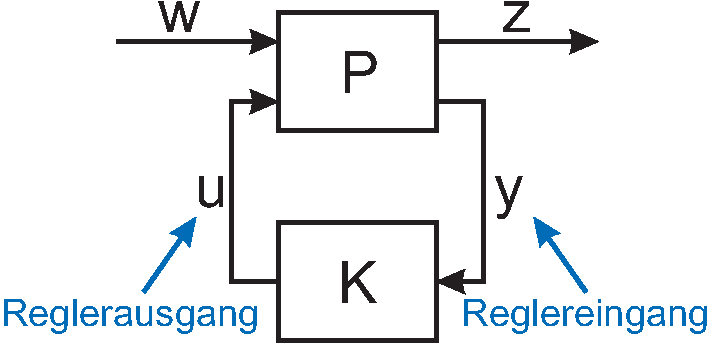
\includegraphics[width=0.8\columnwidth]{Grafiken/PK-Struktur}
\end{center}
\begin{tabular}{p{1cm}p{8cm}}
$P$: & Verallgemeinerte Strecke\\
$K$: & Regler\\
$w$: & Exogener Eingang (z.B. Referenzsignale, Rauschen, Störungen)\\
$z$: & Exogener Ausgang (stellt nicht den Ausgang der Strecke $G(s)$ dar, sondern das Performanzsignal, das durch den Regler angepasst werden soll)\\
$y$: & Reglereingang
\end{tabular}\\\\\\
\textbf{Ziel:}\\
Performanz von $N$ soll garantiert werden mit stabilisierendem Regler $K$.

\subsubsection{Analyse der verallgemeinerten Strecke im Laplace-Bereich}
\textbf{Vorgehen zum Erhalten der PK-Struktur:}
\begin{enumerate}
\item Sammeln aller Signale, die von außen auf das System wirken, in dem Vektor $w$.
\item Bestimmen von $z$ in Abhängigkeit von allen Eingängen, die in $w$ zusammengefasst sind.
\item Bestimmen von $y$ in Abhängigkeit aller Eingänge, die in $w$ zusammengefasst sind. Dann gilt $u=Ky$.
\item Bestimmen der verallgemeinerten Strecke $P$ durch
\begin{align*}
\begin{bmatrix}z \\ y\end{bmatrix}=P\begin{bmatrix}w \\ u\end{bmatrix}
\end{align*}
\end{enumerate}
Oftmals wird $P$ partitioniert in:
\begin{align*}
P=\begin{bmatrix}P_{11} & P_{12} \\ P_{21} & P_{22}\end{bmatrix}
\end{align*}
sodass gilt:
\begin{align*}
z&=P_{11}w+P_{12}u\\
y&=P_{21}w+P_{22}u
\end{align*}
Weiterhin gilt:
\begin{align*}
z&=Nw\\
u&=Ky\\
\Rightarrow N&=P_{11}+P_{12}K(I-P_{22}K)^{-1}P_{21}:=F_l(P,K)=P\star K
\end{align*}

\subsubsection{Beschreibung der verallgemeinerten Strecke im Zeitbereich}
Die Zustandsraumdarstellung für $P$ lautet:
\begin{align*}
\dot{x}&=Ax+B_1w+B_2u\\
z&=C_1x+D_{11}w+D_{12}u\\
y&=C_2x+D_{21}w+D_{22}u
\end{align*}
$K$ kann beschrieben werden durch:
\begin{align*}
\dot{x}_K&=A_Kx+B_Ky\\
u&=C_Kx_K+D_Ky
\end{align*}
falls eine LTI-Reglerdynamik erlaubt ist. Für einen statischen Regler $F$ zur Zustandsrückführung gilt:
\begin{align*}
u=Fx
\end{align*}

\subsubsection{Mixed sensitivity design}
Um ein sinnvolles Reglersyntheseproblem zu erhalten, ist es notwendig, ein gewichtetes Eingangssignal $\tilde{w}(s)=W_w(s)w(s)$ und ein gewichtetes Ausgangssignal $\tilde{z}(s)=W_z(s)z(s)$ einzuführen.
\begin{center}
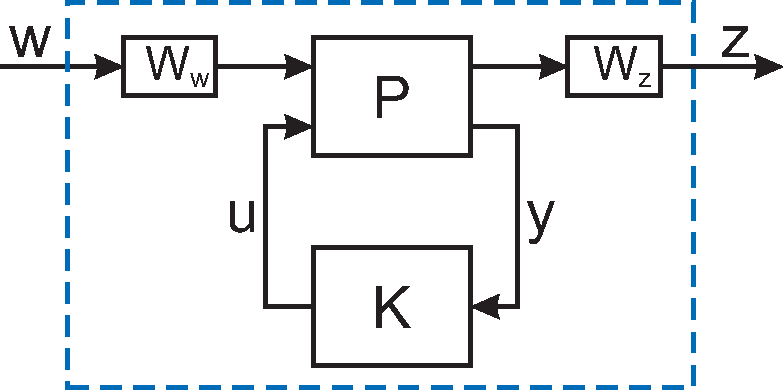
\includegraphics[width=0.8\columnwidth]{Grafiken/PK-Struktur_mit_Gewichten}
\end{center}

\subsection{$H_{\infty}$-optimale Reglersynthese}
Das Standard $H_{\infty}$-Reglerproblem ist der Versuch, einen stabilisierenden Regler $K$ für eine gegebene Strecke $P$ zu finden.\\
Die vorgegebene Performanz wird eingehalten, wenn gilt:
\begin{align*}
||N||_{\infty}<1
\end{align*}
Ziel ist es, die Optimierungsfunktion $||N||_{\infty}$ zu minimieren.\\\\
Das suboptimale Reglersynthesproblem lautet:\\
Finde
\begin{align*}
||N||_{\infty}<\gamma
\end{align*}
sodass $K$ die Strecke $P$ stabilisiert.

\section{Appendix}
\subsection{Singulärwertzerlegung}
Gegeben sei eine Matrix $A\in\mathbb{R}^{m\times n}$. Die Singulärwertzerlegung $A=U\Sigma V^T$ wird wie folgt berechnet:
\begin{enumerate}
\item Berechne
\begin{align*}
B=A^TA
\end{align*}
\item Berechne die nicht-negativen EW von $B$:
\begin{align*}
det(\lambda_iI-B)=0
\end{align*}
und nummeriere sie in der Reihenfolge
\begin{align*}
\lambda_1\geq\lambda_2\geq ...\geq\lambda_n\geq 0
\end{align*}
\item Berechne $v_1,v_2,...,v_n$:
\begin{align*}
(\lambda_iI-B)\tilde{v}_i&=0\\
v_i&=\frac{1}{|\tilde{v}_i|}\cdot\tilde{v}_i\\
V&=[v_1,...,v_n]
\end{align*}
\item Die Singulärwerte berechnen sich wie folgt:
\begin{align*}
\sigma_{ii}&=\sqrt{\lambda_i};\;\;\;i=1,2,...,k=min(m,n)
\end{align*}
\item Berechne $u_1,u_2,...,u_m$:
\begin{align*}
u_i=\frac{1}{\sigma_i}Av_i
\end{align*}
Falls $m>n$ oder falls $\sigma_i=0$, müssen die Vektoren zu einer Orthonormalbasis ergänzt werden.
\begin{align*}
U=(u_1,u_2,...,u_m)
\end{align*}
\end{enumerate}
\vspace{1cm}
Lizenz: CC BY-NC-SA 3.0\\
\url{http://creativecommons.org/licenses/by-nc-sa/3.0/de/}

\end{document}








